\chapter{Physik}

Für die Physik nutzt die Engine innerhalb des \textprog{PhysicsCore}s die \textbf{\href{http://code.google.com/p/box2dweb/}{box2dweb}}\footnote{Projektwebsite unter \url{http://code.google.com/p/box2dweb/}}-Bibliothek, ein Javascript-Port der C++-Bibliothek \textbf{\href{http://box2d.org/}{Box2D}}\footnote{Projektwebsite unter \url{http://box2d.org/}}. Der \textprog{PhysicsCore} erzeugt eine eigene Physik-Welt, innerhalb welcher die Physik-Objekte leben.

\section{Plugin\_PhysicsBox}

Der Großteil der Spielobjekte besitzt eine einfache rechteckige Form - die Böden und Hindernisse der Spielwelt, Trigger und Ähnliches. Um für solche Objekte das Hinzufügen von Physik zu erleichtern, habe ich ein einfaches Plugin, das \textprog{Plugin\_PhysicsBox} geschrieben, welches lediglich dem Spiel-Objekt hinzugefügt werden muss um diesem physikalische Eigenschaften zu geben. Das Plugin holt sich Position (\textprog{pos}), Rotation (\textprog{rot}) und Größe (\textprog{size}) vom zugewiesenen Spielobjekt (basierend auf den Eigenschaften des \textprog{Plugin\_WorldObject3D}) und kümmert sich um die Synchronisation von physikalischer Position und Position des Spielobjekts. Gleiches gilt für die Rotation

Bei Erstellung des Plugins können physikalische Eigenschaften wie Reibung festgelegt werden, ebenso ob es ein statisches oder dynamisches Objekt bzw ein Sensor (registriert Überschneidungen, aber kollidiert nicht) ist.

\newpage
\section{Kollisionen}

Innerhalb von box2dweb gibt es die Möglichkeit einen eigenen \textprog{ContactListener} zu schreiben und der Physik-Welt zuzuordnen um physikalische Kollisionen selbst auszuwerten. Der \textprog{ContactListener} muss Funktionen für die Auswertung der 4 Phasen einer Kollision implementieren:

\begin{itemize}
\item beginContact
\item endContact
\item preSolve
\item postSolve
\end{itemize}


Egal welche Objekte miteinander kollidieren, es werden jeweils genau diese 4 Funktionen aufgerufen. Damit die Spiellogik über Kollisionen informiert wird, sind die Funktionen so implementiert, dass sie für die beiden beteiligten Physik-Objekte die entsprechende Funktion (z. B. \textprog{onBeginContact}) aufrufen, sofern diese vom Spiellogik-Programmierer bereit gestellt wurde. Innerhalb dieses Aufrufs kann dann die Kollision ausgewertet werden. Möglich ist dies nur dadurch, dass man innerhalb von Javascript jedem Objekt beliebige Eigenschaften und Funktionen hinzufügen kann.

\begin{lstlisting}[language=JavaScript, caption=\textprog{BeginContact}-Methode des von mir bereitgestellten ContactListeners]
BeginContact: function BeginContact(contact)
{
	var fixA = contact.GetFixtureA();
	var fixB = contact.GetFixtureB();
	
	if(fixA.onBeginContact)
		fixA.onBeginContact(fixA, fixB, contact);
		
	if(fixB.onBeginContact)
		fixB.onBeginContact(fixB, fixA, contact);
},
\end{lstlisting}

\section{Probleme}

Aktuell gibt es noch einen Grafik-Bug, welcher mit der Physik zu tun hat. So liegen dynamische Physik-Objekte oft nicht direkt auf anderen Physik-Objekten auf - es gibt Lücken. Diese resultieren daher, dass Box2D eine kleine Schutzschicht um dynamische Objekte legt um Tunneling zu verhindern. So berühren sich diese Objekte an sich nie direkt, welches sich selbstverständlich in der grafischen Repräsentation niederschlägt.

\begin{figure}[h] % h = here
	\centering
		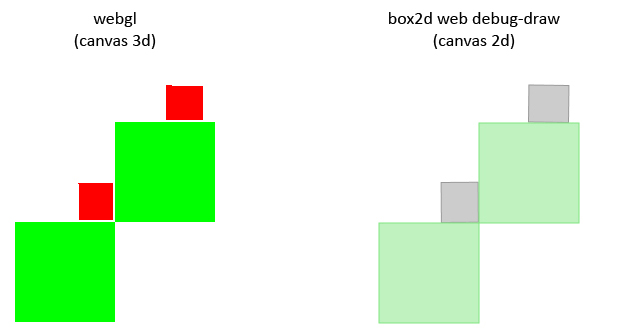
\includegraphics[scale=0.6]{images/gap_bug.jpg}
	\caption{Lücken-Bug: links WebGL, rechts box2dweb debug-view}
\end{figure}

Eine Möglichkeit zur Lösung dieses Problems, wäre es die Grafikobjekte leicht größer zu zeichnen als sie sind. Box2D bietet zudem eine Eigenschaft, mit der festgestellt werden kann, wie groß die Schutzschicht um ein dynamisches Physik-Objekt herum ist. Basierend darauf könnte man die zu zeichnende Größe des Grafik-Objekts bestimmen. Diese Aufgabe wurde jedoch noch nicht erledigt.

\subsection{Anti-Aliasing}

Bei Überprüfung dieses Lücken-Zustandes in der box2dweb-Debug-Ansicht (siehe Screenshot), sieht es so aus, als ob die Lücken dort kleiner wären. Dies hat damit zu tun, dass dort ein 2D-\textprog{canvas}-Kontext genutzt wird, bei dem - im Gegensatz zu WebGL - anti-aliasing aktiviert ist.

